\title{Generative Adversarial Networks}

\subsection{Generative Adversarial Networks}

Generative adversarial networks (GANs) are a powerful approach for
probabilistic modeling \citep{goodfellow2014generative,goodfellow2016nips}.
They posit a deep generative model and they enable fast and accurate
inferences.

We demonstrate with an example in Edward.
An interactive version with Jupyter notebook is available
\href{http://nbviewer.jupyter.org/github/blei-lab/edward/blob/master/docs/notebooks/gan.ipynb}{here},
or as a script available at
\href{https://github.com/blei-lab/edward/blob/master/examples/gan.py}
{\texttt{examples/gan.py}} in the Github repository.

\begin{lstlisting}[language=Python]
M = 128  # batch size during training
d = 100  # latent dimension

DATA_DIR = "data/mnist"
IMG_DIR = "img"
\end{lstlisting}

\subsubsection{Data}

We use training data from MNIST, which consists of 55,000 $28\times
28$ pixel images \citep{lecun1998gradient}. Each image is represented
as a flattened vector of 784 elements, and each element is a pixel
intensity between 0 and 1.

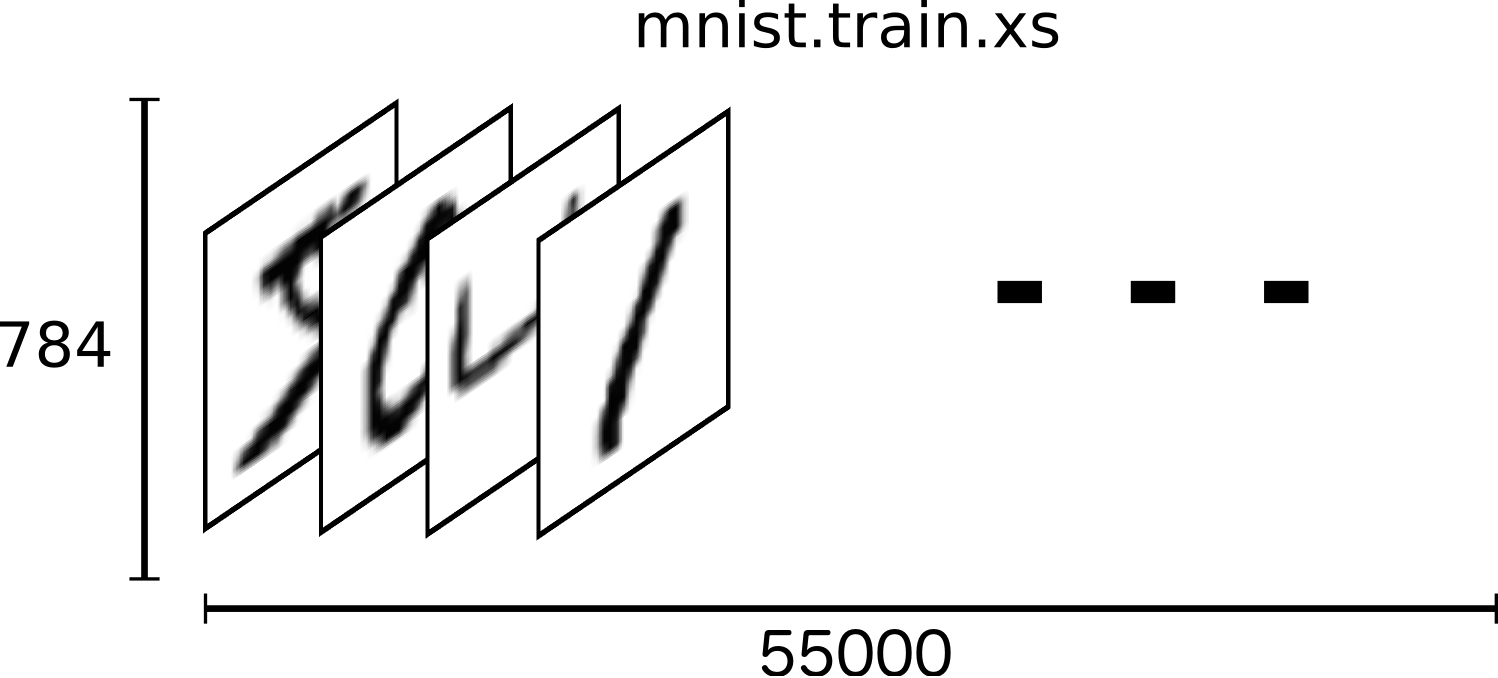
\includegraphics[width=450px]{/images/gan-fig0.png}

The goal is to build and infer a model that can generate high quality
images of handwritten digits.

During training we will feed batches of MNIST digits. We instantiate a
TensorFlow placeholder with a fixed batch size of $M$ images.

\begin{lstlisting}[language=Python]
from tensorflow.examples.tutorials.mnist import input_data

mnist = input_data.read_data_sets(DATA_DIR, one_hot=True)
x_ph = tf.placeholder(tf.float32, [M, 784])
\end{lstlisting}


\subsubsection{Model}

GANs posit generative models using an implicit mechanism. Given some
random noise, the data is assumed to be generated by a deterministic
function of that noise.

Formally, the generative process is
\begin{align*}
\mathbf{\epsilon} &\sim p(\mathbf{\epsilon}), \\
\mathbf{x} &= G(\mathbf{\epsilon}; \theta),
\end{align*}
where $G(\cdot; \theta)$ is a neural network that takes the samples
$\mathbf{\epsilon}$ as input. The distribution
$p(\mathbf{\epsilon})$ is interpreted as random noise injected to
produce stochasticity in a physical system; it is typically a fixed
uniform or normal distribution with some latent dimensionality.

In Edward, we build the model as follows, using TensorFlow Slim to
specify the neural network. It defines a 2-layer fully connected neural
network and outputs a vector of length $28\times28$ with values in
$[0,1]$.

\begin{lstlisting}[language=Python]
from edward.models import Uniform
from tensorflow.contrib import slim

def generative_network(eps):
  h1 = slim.fully_connected(eps, 128, activation_fn=tf.nn.relu)
  x = slim.fully_connected(h1, 784, activation_fn=tf.sigmoid)
  return x

with tf.variable_scope("Gen"):
  eps = Uniform(a=tf.zeros([M, d]) - 1.0, b=tf.ones([M, d]))
  x = generative_network(eps)
\end{lstlisting}

We aim to estimate parameters of the generative network such
that the model best captures the data. (Note in GANs, we are
interested only in parameter estimation and not inference about any
latent variables.)

Unfortunately, probability models described above do not admit a tractable
likelihood. This poses a problem for most inference algorithms, as
they usually require taking the model's density.  Thus we are
motivated to use ``likelihood-free'' algorithms
\citep{marin2012approximate}, a class of methods which assume one
can only sample from the model.

\subsubsection{Inference}

A key idea in likelihood-free methods is to learn by
comparison (e.g., \citet{rubin1984bayesianly,gretton2012kernel}): by
analyzing the discrepancy between samples from the model and samples
from the true data distribution, we have information on where the
model can be improved in order to generate better samples.

In GANs, a neural network $D(\cdot;\phi)$ makes this comparison,
known as the discriminator.
$D(\cdot;\phi)$ takes data $\mathbf{x}$ as input (either
generations from the model or data points from the data set), and it
calculates the probability that $\mathbf{x}$ came from the true data.

In Edward, we use the following discriminative network. It is simply a
feedforward network with one ReLU hidden layer. It returns the
probability in the logit (unconstrained) scale.

\begin{lstlisting}[language=Python]
def discriminative_network(x):
  h1 = slim.fully_connected(x, 128, activation_fn=tf.nn.relu)
  logit = slim.fully_connected(h1, 1, activation_fn=None)
  return logit
\end{lstlisting}

Let $p^*(\mathbf{x})$ represent the true data distribution.
The optimization problem used in GANs is

\begin{equation*}
\min_\theta \max_\phi~
\mathbb{E}_{p^*(\mathbf{x})} [ \log D(\mathbf{x}; \phi) ]
+ \mathbb{E}_{p(\mathbf{x}; \theta)} [ \log (1 - D(\mathbf{x}; \phi)) ].
\end{equation*}

This optimization problem is bilevel: it requires a min-max solution.
In practice, the algorithm proceeds by iterating among these two
optimizations, alternating gradient updates. An
additional heuristic also modifies the objective function for the
generative model in order to avoid saturation of gradients
\citep{goodfellow2014on}.

Many sources of intuition exist behind GAN-style training. One, which
is the original motivation, is based on idea that the two neural
networks are playing a game. The discriminator tries to best
distinguish samples away from the generator. The generator tries
to produce samples that are indistinguishable by the discriminator.
The goal of training is to reach a Nash equilibrium.

Another source is the idea of casting unsupervised learning as
supervised learning
\citep{gutmann2010noise,gutmann2014statistical}.
This allows one to leverage the power of classification—a problem that
in recent years is (relatively speaking) very easy.

A third comes from classical statistics, where the discriminator is
interpreted as a proxy of the density ratio between the true data
distribution and the model
\citep{sugiyama2012density,mohamed2016learning}. By augmenting an
original problem that may require the model's density with a
discriminator (such as maximum likelihood), one can recover the
original problem when the discriminator is optimal. Furthermore, this
approximation is very fast, and it justifies GANs from the perspective
of approximate inference.

In Edward, the GAN algorithm (\texttt{GANInference}) simply takes the
implicit density model on \texttt{x} as input, binded to its
realizations \texttt{x_ph}. In addition, a parameterized function
\texttt{discriminator} is provided to distinguish their
samples.

\begin{lstlisting}[language=Python]
inference = ed.GANInference(
    data={x: x_ph}, discriminator=discriminative_network)
\end{lstlisting}

We'll use ADAM as optimizers for both the generator and discriminator.
We'll run the algorithm for 15,000 iterations and print progress every
1,000 iterations.

\begin{lstlisting}[language=Python]
optimizer = tf.train.AdamOptimizer()
optimizer_d = tf.train.AdamOptimizer()

inference.initialize(
    optimizer=optimizer, optimizer_d=optimizer,
    n_iter=15000, n_print=1000)
\end{lstlisting}

We now form the main loop which trains the GAN. At each iteration, it
takes a minibatch and updates the parameters according to the
algorithm. At every 1000 iterations, it will print progress. It also
saves a figure of generated samples from the model.

\begin{lstlisting}[language=Python]
sess = ed.get_session()
tf.global_variables_initializer().run()

idx = np.random.randint(M, size=16)
i = 0
for t in range(inference.n_iter):
  if t % inference.n_print == 0:
    samples = sess.run(x)
    samples = samples[idx, ]

    fig = plot(samples)
    plt.savefig(os.path.join(IMG_DIR, '{}.png').format(
        str(i).zfill(3)), bbox_inches='tight')
    plt.close(fig)
    i += 1

  x_batch, _ = mnist.train.next_batch(M)
  info_dict = inference.update(feed_dict={x_ph: x_batch})
  inference.print_progress(info_dict)
\end{lstlisting}

Examining convergence of the GAN objective can be meaningless in
practice. The algorithm is usually run until some other criterion is
satisfied, such as if the samples look visually okay, or if the GAN
can capture meaningful parts of the data.

\subsubsection{Criticism}

Evaluation of GANs remains an open problem---both in criticizing their
fit to data and in assessing convergence.
Recent advances have considered alternative objectives and
heuristics to stabilize training (see also Soumith Chintala's
\href{https://github.com/soumith/ganhacks}{GAN hacks repo}).

As one approach to criticize the model, we simply look at generated
images during training. Below we show generations after 14,000
iterations (that is, 14,000 gradient updates of both the generator and
the discriminator).

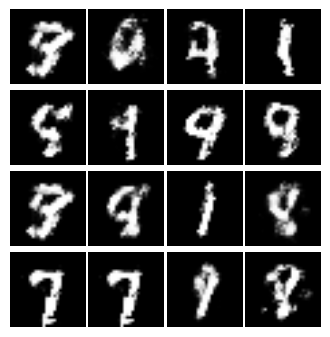
\includegraphics[width=500px]{/images/gan-fig1.png}

The images are meaningful albeit a little blurry. Suggestions for
further improvements would be to tune the hyperparameters in the
optimization, to improve the capacity of the discriminative and
generative networks, and to leverage more prior information (such as
convolutional architectures).

\subsubsection{References}\label{references}
